\apendice{Especificación de Requisitos}

\section{Introducción}

En esta sección se recoge la especificación de requisitos que define el comportamiento del sistema desarrollado.
Esta sección tiene como objetivo documentar correctamente la forma en la que se ha desarrollado PrimeBot.

Se han seguido las recomendaciones del estándar IEEE 830-1998 que manifiesta que una buena especificación de requisitos de software debe ser:

\begin{itemize}
\tightlist
\item
  \textbf{Completa}: todos los requerimientos deben estar reflejados en
  ella y todas las referencias deben estar definidas.
\item
  \textbf{Consistente}: debe ser coherente con los propios
  requerimientos y también con otros documentos de especificación.
\item
  \textbf{Inequívoca}: la redacción debe ser clara de modo que no se
  pueda mal interpretar.
\item
  \textbf{Correcta}: el software debe cumplir con los requisitos de la
  especificación.
\item
  \textbf{Trazable}\emph{: s}e refiere a la posibilidad de verificar la
  historia, ubicación o aplicación de un ítem a través de su
  identificación almacenada y documentada.
\item
  \textbf{Priorizable}: los requisitos deben poder organizarse
  jerárquicamente según su relevancia para el negocio y clasificándolos
  en esenciales, condicionales y opcionales.
\item
  \textbf{Modificable}: aunque todo requerimiento es modificable, se
  refiere a que debe ser fácilmente modificable.
\item
  \textbf{Verificable}: debe existir un método finito sin costo para
  poder probarlo.
\end{itemize}

\section{Objetivos generales}
El proyecto persigue los siguientes objetivos generales:

\begin{itemize}
\tightlist
\item
  Desarrollar una algoritmo PID eficiente y de alto rendimiento para seguir línea negra.
\item
  Implementar un algoritmo para la resolución de la prueba de cuadrícula.
\item
  Implementar un algoritmo eficiente para la resolución de laberintos.
\item
  Establecer protocolos de comunicación Bluetooth a tiempo real para aumentar el rendimiento de PrimeBot.
  \item
  Permitir ejecutar varios programas a la vez sin necesidad de un PC.
\end{itemize}

\section{Catálogo de requisitos}\label{catalogo-de-requisitos}

A continuación, se enumeran los requisitos específicos derivados de los objetivos generales del proyecto.
\subsection{Requisitos funcionales}\label{requisitos-funcionales}

\begin{itemize}
\tightlist
\item
  \textbf{RF-1 Seguimiento de línea:} PrimeBot debe ser capaz de seguir líneas negras sobre un fondo blanco utilizando los sensores QTR8A.
  \begin{itemize}
  \tightlist
  \item
    \textbf{RF-1.1 Detección de Líneas:} Los sensores QTR8A detectan el contraste entre la línea negra y el fondo blanco.
  \item
    \textbf{RF-1.2 Ajuste de Dirección:} El algoritmo PID ajusta la dirección del robot basándose en la información de los sensores.
  \item
    \textbf{RF-1.3 Calibración inicial:} antes de comenzar las pruebas, PrimeBot debe calibrar sus sensores QTR8A para seguir correctamente la línea negra.
\end{itemize}
\item
  \textbf{RF-2 Navegacion en cuadricula :} PrimeBot debe moverse de una estación de origen a una estación de destino en una cuadrícula predefinida.
  \begin{itemize}
  \tightlist
  \item
    \textbf{RF-2.1 Detección de Cruces:} El robot detecta los cruces en la cuadrícula utilizando los sensores QTR8A.
  \item
    \textbf{RF-2.2 Cálculo de Rutas:} El robot calcula la ruta más eficiente desde la estación de origen a la de destino.
  \item
    \textbf{RF-2.3 Evitar puntos bloqueados:} PrimeBot debe ser capaz de calcular rutas alternativas ante puntos de la cuadrícula bloqueados.
  \end{itemize}
\item
  \textbf{RF-3 Resolución de laberintos: } PrimeBot debe navegar y resolver laberintos utilizando algoritmos de búsqueda y sensores OPT3101.
  \begin{itemize}
  \tightlist
  \item
    \textbf{RF-3.1 Detección de Paredes: } Los sensores OPT3101 detectan la presencia de paredes en el laberinto.
  \item
    \textbf{RF-3.2 Detección de huecos: } PrimeBot debe ser capaz de detectar los huecos que hay en el laberinto para navegar sobre él.
  \end{itemize}

\end{itemize}

\subsection{Requisitos no funcionales}\label{requisitos-no-funcionales}
\begin{itemize}
\tightlist
\item
\textbf{RNF-1 Rendimiento:} PrimeBot debe operar con un tiempo de respuesta mínimo y eficiente.
\item
\textbf{RNF-2 Confiabilidad:} PrimeBot debe ser confiable y operar sin fallos durante largos periodos.
\item
\textbf{RNF-3 Usabilidad:} PrimeBot debe ser fácil de usar e interactuar.

\begin{itemize}
\tightlist
\item
\textbf{RNF-3.1 Interfaz de Usuario:} El robot debe ser controlable mediante una interfaz de usuario sencilla y los ajustes vía Bluetooth deben ser intuitivos.
\end{itemize}
\item
\textbf{RNF-4 Mantenibilidad:} El código y hardware de PrimeBot deben ser fáciles de mantener y actualizar.

\begin{itemize}
\tightlist
\item
\textbf{RNF-4.1 Actualización de Software y Hardware:} Las actualizaciones deben poder realizarse sin necesidad de una reestructuración completa.
\end{itemize}
\item
\textbf{RNF-5 Portabilidad:} PrimeBot debe ser portátil y fácil de transportar.

\begin{itemize}
\tightlist
\item
\textbf{RNF-5.1 Peso y Dimensiones:} El robot debe ser ligero y compacto, con un peso inferior a 1 kg y dimensiones manejables.
\end{itemize}
\item
\textbf{RNF-6 Escalabilidad:} PrimeBot debe permitir futuras expansiones y mejoras.

\begin{itemize}
\tightlist
\item
\textbf{RNF-6.1 Adición de Nuevos Componentes:} La arquitectura debe permitir la adición de nuevos sensores y módulos sin necesidad de un rediseño significativo.
\end{itemize}
\item
\textbf{RNF-7 Seguridad:} PrimeBot debe operar de manera segura tanto para los usuarios como para el entorno.
\end{itemize}

\newpage
\section{Diagramas UML}

\subsection{Diagrama de flujo}

A continuación se muestra un diagrama de flujo de la selección de programa de PrimeBot (Figura B.1).
Esta selección se realiza con el selector DIP y el pulsador que hay en la parte trasera del PCB de PrimeBot

\begin{figure}[h]
	\centering
	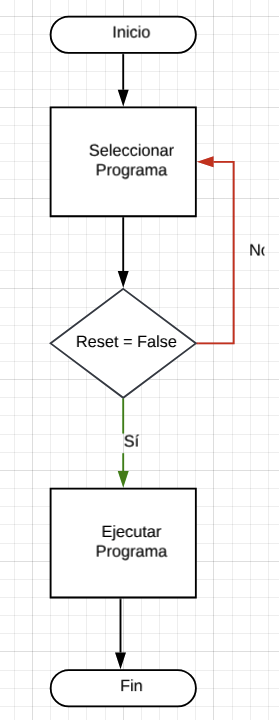
\includegraphics[width=0.25\textwidth]{anexos/diagramaDeFlujo}
	\caption{Diagrama de Flujo.}
	\label{fig:B.1}
\end{figure}
\newpage
\subsection{Diagramas de secuencias}
A continuación se colocan los diagramas de secuencias de las diferentes pruebas que realiza PrimeBot.
\subsubsection{Prueba de siguelineas}
La prueba de siguelíneas se realiza de forma ininterrumpida hasta que se vuelve a pulsar el botón con otro programa seleccionado (Figura B.2).
\begin{figure}[h]
	\centering
	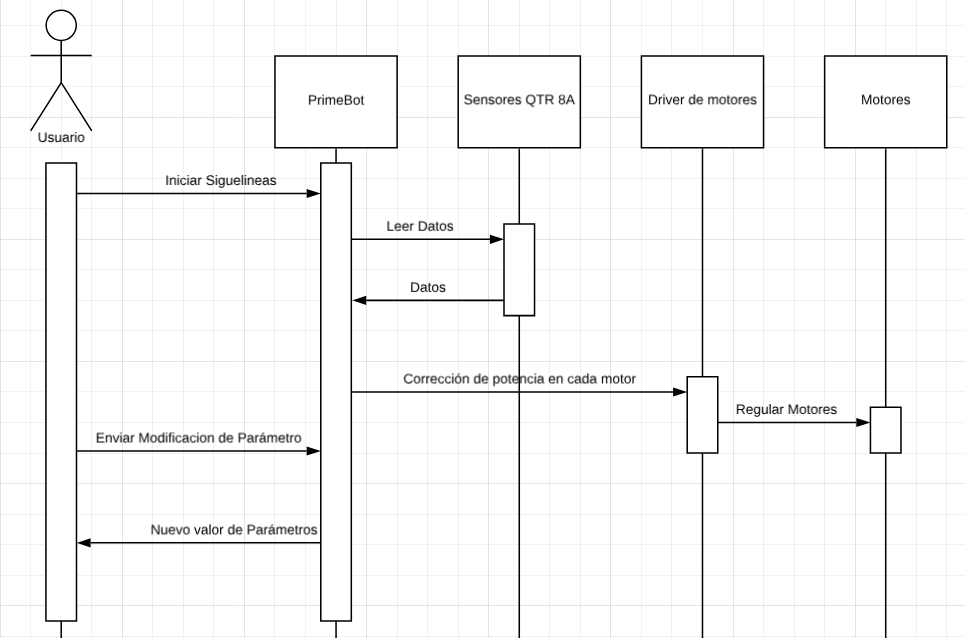
\includegraphics[width=0.5\textwidth]{anexos/diagramaSiguelineas}
	\caption{Diagrama de secuencia programa siguelineas.}
	\label{fig:B.2}
\end{figure}

\subsubsection{Prueba de cuadrícula}

La prueba de la cuadrícula es la más compleja y se realiza a partir de unos argumentos que el usuario aporta a PrimeBot.

En el diagra de secuencias se puede ver la ejecución completa del programa (Figura B.3).

\begin{figure}[h]
	\centering
	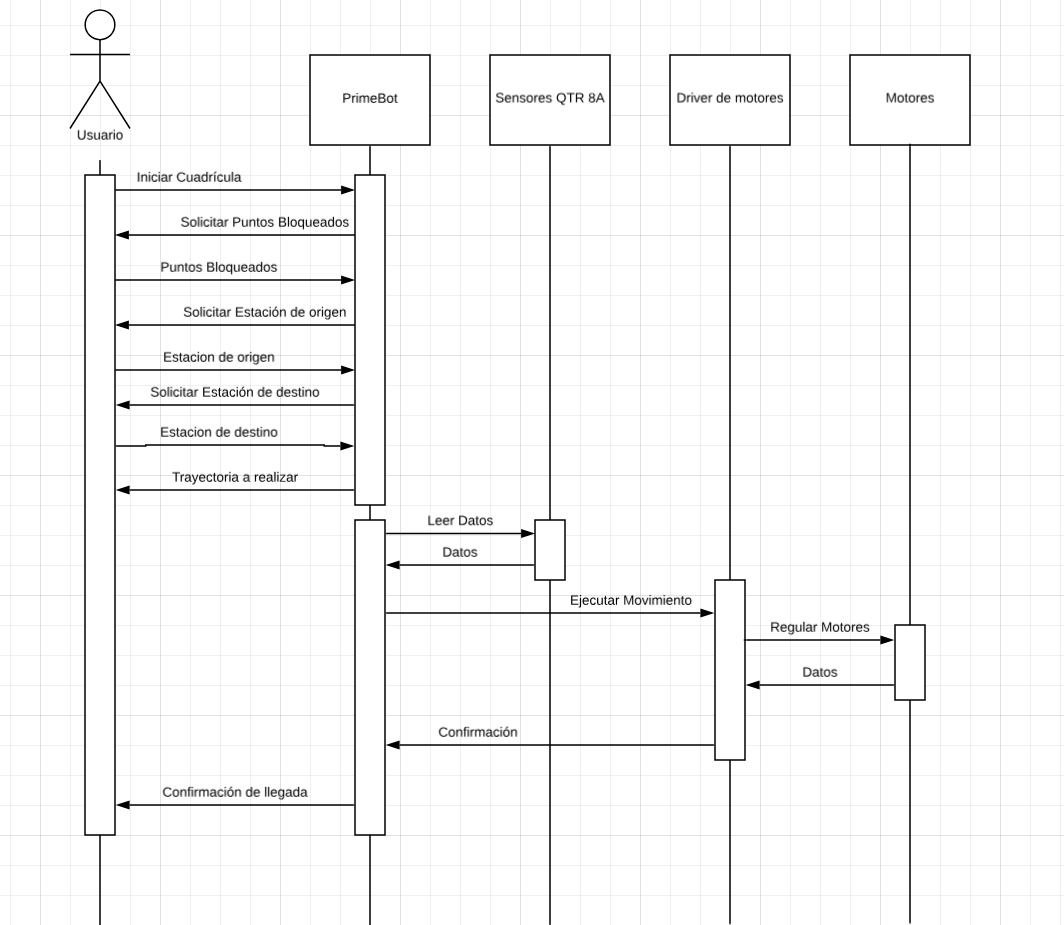
\includegraphics[width=0.5\textwidth]{anexos/diagramaCuadricula}
	\caption{Diagrama de secuencia programa de resolución de cuadrícula.}
	\label{fig:B.3}
\end{figure}
\newpage
\subsubsection{Prueba de laberinto}

\begin{figure}[h]
	\centering
	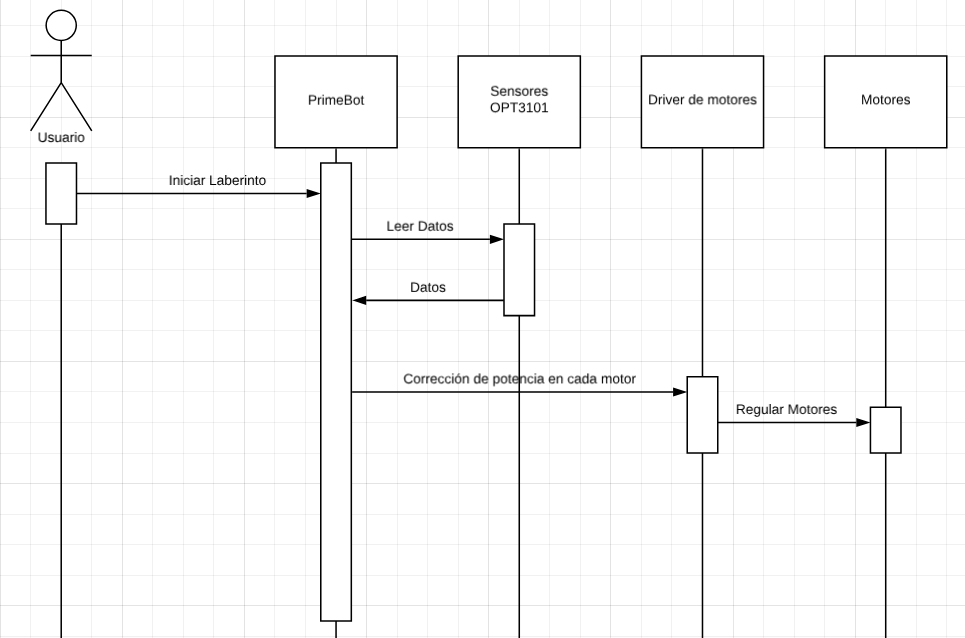
\includegraphics[width=0.5\textwidth]{anexos/diagramaLaberinto}
	\caption{Diagrama de secuencia programa de resolución de laberinto.}
	\label{fig:B.2}
\end{figure}


\newpage
\section{Especificación de requisitos}

En esta sección se desarrollará cada caso de uso del sistema.
\begin{table}[p]
	\centering
	\begin{tabularx}{\linewidth}{ p{0.21\columnwidth} p{0.71\columnwidth} }
		\toprule
		\textbf{CU-1}    & \textbf{Calibración de Sensores}\\
		\toprule
		\textbf{Versión}              & 1.0    \\
		\textbf{Autor}                & Mario Alonso Pulgar \\
		\textbf{Requisitos asociados} & RF-1.3 \\
		\textbf{Descripción}          & PrimeBot calibra sus sensores QTR para una mejor precisión en el seguimiento de líneas.\\
		\textbf{Precondición}         & PrimeBot está encendido y los sensores QTR están conectados.\\
		\textbf{Acciones}             &
		\begin{enumerate}
			\def\labelenumi{\arabic{enumi}.}
			\tightlist
			\item El usuario selecciona la opción de calibración en el dip-switch.
			\item PrimeBot enciende los LEDs de calibración.
			\item PrimeBot calibra los sensores durante 400 iteraciones.
			\item PrimeBot apaga los LEDs de calibración.
		\end{enumerate}\\
		\textbf{Postcondición}        & Los sensores QTR están calibrados y listos para su uso.  \\
		\textbf{Excepciones}          & Si la calibración falla, PrimeBot avisa al usuario y detiene la operación.  \\
		\textbf{Importancia}          & Alta \\
		\bottomrule
	\end{tabularx}
	\caption{CU-1 Calibración de Sensores.}
\end{table}

% Caso de Uso 1 -> Consultar Experimentos.
\begin{table}[p]
	\centering
	\begin{tabularx}{\linewidth}{ p{0.21\columnwidth} p{0.71\columnwidth} }
		\toprule
		\textbf{CU-2}    & \textbf{Seguimiento de linea}\\
		\toprule
		\textbf{Versión}              & 1.0    \\
		\textbf{Autor}                & Mario Alonso Pulgar \\
		\textbf{Requisitos asociados} & RF-1, RF-1.1, RF-1.2\\
		\textbf{Descripción}          & PrimeBot sigue una línea negra sobre un fondo blanco utilizando los sensores QTR8A.\\
		\textbf{Precondición}         & PrimeBot está encendido, los sensores QTR8A están calibrados y está seleccionado el programa 0001\\
		\textbf{Acciones}             &
		\begin{enumerate}
			\def\labelenumi{\arabic{enumi}.}
			\tightlist
				\item El usuario coloca PrimeBot al inicio de una línea negra.
				\item PrimeBot detecta la línea utilizando los sensores QTR8A.
				\item PrimeBot ajusta su dirección mediante el algoritmo PID.
				\item PrimeBot sigue la línea hasta el final del recorrido.
		\end{enumerate}\\
		\textbf{Postcondición}        & PrimeBot sigue la línea negra sin salirse del camino.  \\
		\textbf{Excepciones}          & Si PrimeBot pierde la línea, recalibra los sensores y vuelve a buscar la línea.  \\
		\textbf{Importancia}          & Alta \\
		\bottomrule
	\end{tabularx}
	\caption{CU-2 Seguimiento de Líneas.}
\end{table}

\begin{table}[p]
	\centering
	\begin{tabularx}{\linewidth}{ p{0.21\columnwidth} p{0.71\columnwidth} }
		\toprule
		\textbf{CU-3}    & \textbf{Navegación en Cuadrícula}\\
		\toprule
		\textbf{Versión}              & 1.0    \\
		\textbf{Autor}                & Mario Alonso Pulgar \\
		\textbf{Requisitos asociados} & RF-2, RF-2.1, RF-2.2, RF-2.3 \\
		\textbf{Descripción}          & PrimeBot se mueve de una estación de origen a una estación de destino en una cuadrícula predefinida.\\
		\textbf{Precondición}         & PrimeBot está encendido, los sensores QTR8A están calibrados y está seleccionado el programa 0010\\
		\textbf{Acciones}             &
		\begin{enumerate}
			\def\labelenumi{\arabic{enumi}.}
			\tightlist
				\item El usuario indica las estaciones de origen y destino a través de Bluetooth.
				\item PrimeBot detecta los cruces en la cuadrícula utilizando los sensores QTR8A.
				\item PrimeBot calcula la ruta más eficiente.
				\item PrimeBot se mueve a través de la cuadrícula hasta llegar a la estación de destino.
		\end{enumerate}\\
		\textbf{Postcondición}        & PrimeBot llega a la estación de destino. \\
		\textbf{Excepciones}          & Si PrimeBot pierde la línea, recalibra los sensores y vuelve a buscar la línea.  \\
		\textbf{Importancia}          & Alta \\
		\bottomrule
	\end{tabularx}
	\caption{CU-3 Navegación en Cuadrícula.}
\end{table}

\begin{table}[p]
	\centering
	\begin{tabularx}{\linewidth}{ p{0.21\columnwidth} p{0.71\columnwidth} }
		\toprule
		\textbf{CU-4}    & \textbf{Resolución de Laberintos}\\
		\toprule
		\textbf{Versión}              & 1.0    \\
		\textbf{Autor}                & Mario Alonso Pulgar \\
		\textbf{Requisitos asociados} & RF-3, RF-3.1, RF-3.2 \\
		\textbf{Descripción}          & PrimeBot navega y resuelve laberintos utilizando algoritmos de búsqueda y sensores OPT3101. \\
		\textbf{Precondición}         & PrimeBot está encendido, los sensores OPT3101 están calibrados y está seleccionado el programa 0011\\
		\textbf{Acciones}             &
		\begin{enumerate}
			\def\labelenumi{\arabic{enumi}.}
			\tightlist
				\item El usuario coloca PrimeBot en la entrada del laberinto.
				\item PrimeBot utiliza los sensores OPT3101 para detectar paredes.
				\item PrimeBot emplea un algoritmo de búsqueda para planificar su ruta.
				\item PrimeBot navega a través del laberinto.
				\item PrimeBot llega a la salida del laberinto.
		\end{enumerate}\\
		\textbf{Postcondición}        & PrimeBot encuentra la salida del laberinto.\\
		\textbf{Excepciones}          & Si PrimeBot encuentra un obstáculo inesperado, recalcula la ruta y continúa navegando. \\
		\textbf{Importancia}          & Alta \\
		\bottomrule
	\end{tabularx}
	\caption{CU-4 Resolución de Laberintos}
\end{table}

\begin{table}[p]
	\centering
	\begin{tabularx}{\linewidth}{ p{0.21\columnwidth} p{0.71\columnwidth} }
		\toprule
		\textbf{CU-5}    & \textbf{Ajuste de Parámetros PID}\\
		\toprule
		\textbf{Versión}              & 1.0    \\
		\textbf{Autor}                & Mario Alonso Pulgar \\
		\textbf{Requisitos asociados} & RNF-3 \\
		\textbf{Descripción}          & El usuario ajusta los parámetros del controlador PID para optimizar el rendimiento de PrimeBot.\\
		\textbf{Precondición}         & PrimeBot está encendido y conectado al sistema de control.\\
		\textbf{Acciones}             &
		\begin{enumerate}
			\def\labelenumi{\arabic{enumi}.}
			\tightlist
			\item El usuario selecciona el parámetro PID a ajustar (Kp, Ki, Kd, Kv).
			\item El usuario incrementa o decrementa el valor del parámetro seleccionado.
			\item PrimeBot ajusta su comportamiento en función del nuevo valor del parámetro PID.
		\end{enumerate}\\
		\textbf{Postcondición}        & Los parámetros PID están ajustados para un rendimiento óptimo.\\
		\textbf{Excepciones}          & Si el ajuste no es satisfactorio, el usuario puede revertir los cambios. \\
		\textbf{Importancia}          & Media \\
		\bottomrule
	\end{tabularx}
	\caption{CU-5 Ajuste de Parámetros PID.}
\end{table}